\documentclass[../main.tex]{subfiles}
\begin{document}
\chapter{Instalasi GUI Turbo Assembler dan Struktur Program}

    \section{Tujuan Pembelajaran}
        Mahasiswa mampu:
        \begin{itemize}
            \item Melakukan instalasi dan konfigurasi GUI Turbo Assembler (GTASM) sebagai \\
            lingkungan pengembangan terintegrasi untuk pemrograman assembly.
            \item Menjelaskan perbedaan struktur dan karakteristik program \texttt{.COM} dan \texttt{.EXE}.
            \item Menggunakan direktif dasar (\texttt{ORG}, \texttt{END}, \texttt{TITLE}, \texttt{PAGE}) dalam berkas ASM.
            \item Menulis, merakit, menautkan, dan menjalankan program assembly sederhana menggunakan GUI Turbo Assembler.
        \end{itemize}

    \section{Pendahuluan}
        GUI Turbo Assembler (GTASM) adalah lingkungan pengembangan terintegrasi (IDE) yang dirancang untuk mempermudah pemrograman bahasa assembly dengan menyediakan antarmuka grafis yang ramah pengguna \cite{borland1990tasm}. GTASM mengintegrasikan Borland Turbo Assembler (TASM), Turbo Linker (TLINK), Turbo Debugger (TD), dan DOSBox dalam satu paket lengkap, sehingga mendukung pengembangan program tingkat rendah pada arsitektur x86 dan x64 \cite{dosbox_manual}. Pemahaman struktur program \texttt{.COM} vs \texttt{.EXE} penting untuk pemilihan model memori, organisasi segmen, dan strategi \textit{build}. GTASM menyediakan fitur modern seperti penyorotan sintaks (\textit{syntax highlighting}), penomoran baris, pelipatan kode (\textit{code folding}), dan personalisasi tema yang memudahkan proses pembelajaran dan pengembangan.

    \section{Instalasi GUI Turbo Assembler}
        \subsection{Persyaratan sistem}
            GUI Turbo Assembler dapat berjalan pada sistem operasi Windows modern (Windows 7, 8, 10, 11) baik versi 32-bit maupun 64-bit. Persyaratan utama:
            \begin{itemize}
\item Microsoft .NET Framework 4.0 atau lebih tinggi
\item Minimal 100 MB ruang penyimpanan untuk instalasi lengkap
\item DOSBox sudah terintegrasi dalam paket instalasi
            \end{itemize}

        \subsection{Proses instalasi}
            \begin{enumerate}
\item Unduh GUI Turbo Assembler dari sumber terbuka:
\begin{itemize}
    \item GitHub: \\
    \url{https://github.com/ljnath/GUI-Turbo-Assembler}
    \item Softpedia: \\
    \url{https://www.softpedia.com/get/Programming/} \\
    \url{Other-Programming-Files/GUI-Turbo-Assembler.shtml}
\end{itemize}
\item Jalankan file instalasi yang telah diunduh (biasanya bernama \texttt{GTASM\_Setup.exe}).
\item Jika muncul peringatan keamanan Windows, klik \textit{``More info''} kemudian \textit{``Run anyway''}.
\item Ikuti wizard instalasi dengan mengklik \textit{``Next''} pada setiap langkah.
\item Pilih direktori instalasi (default: \texttt{C:\\Program Files\\GUI Turbo Assembler}).
\item Centang opsi untuk membuat shortcut di desktop dan menu Start.
\item Klik \textit{``Install''} dan tunggu proses instalasi selesai.
\item Klik \textit{``Finish''} untuk menyelesaikan instalasi.
            \end{enumerate}

            \begin{figure}[H]
\centering
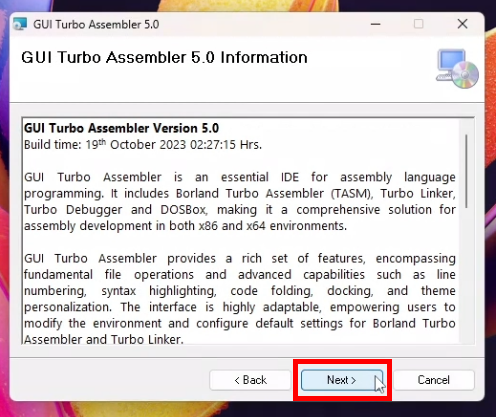
\includegraphics[width=0.8\textwidth]{images/gtasm_installer.png}
\caption{Wizard instalasi GUI Turbo Assembler}
\label{fig:gtasm-installer}
            \end{figure}

            \subsubsection{Verifikasi instalasi}
Setelah instalasi selesai, lakukan verifikasi:
\begin{enumerate}
    \item Buka GUI Turbo Assembler dari shortcut desktop atau menu Start.
    \item Periksa menu \textit{``Help''} $\rightarrow$ \textit{``About''} untuk melihat versi GTASM dan komponen yang terinstal.
    \item Pastikan TASM, TLINK, TD, dan DOSBox sudah terintegrasi dengan baik.
\end{enumerate}

            \subsubsection{Konfigurasi awal}
GUI Turbo Assembler umumnya tidak memerlukan konfigurasi tambahan karena semua komponen sudah terintegrasi. Namun, Anda dapat melakukan personalisasi:
\begin{itemize}
    \item Pilih tema editor melalui menu \textit{``Tools''} $\rightarrow$ \textit{``Options''} $\rightarrow$ \textit{``Theme''}.
    \item Atur ukuran font dan preferensi editor sesuai kenyamanan.
    \item Konfigurasi bahasa antarmuka (mendukung 7 bahasa) melalui menu \textit{``Language''}.
\end{itemize}

        \subsection{Lingkungan Pengembangan GUI Turbo Assembler}
            GUI Turbo Assembler menyediakan lingkungan pengembangan lengkap dengan antarmuka grafis modern:

            \begin{figure}[H]
\centering
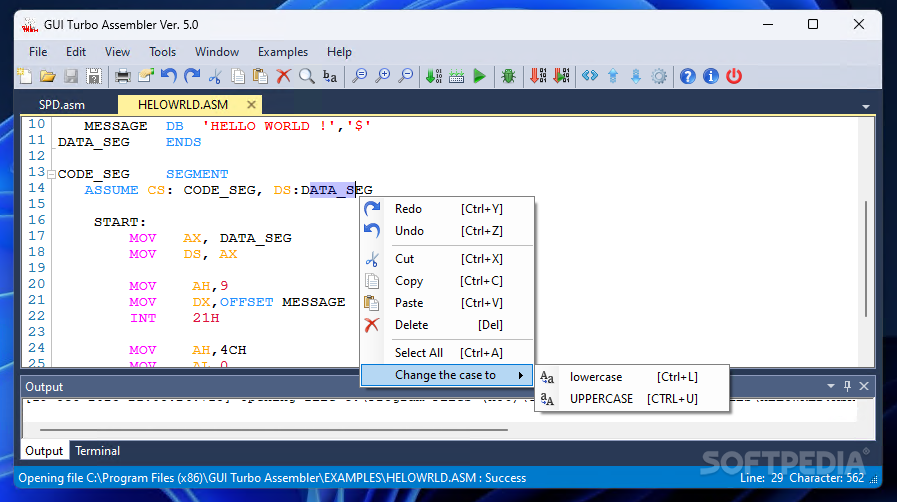
\includegraphics[width=0.75\textwidth]{images/gtasm_interface.png}
\caption{Antarmuka utama GUI Turbo Assembler}
\label{fig:gtasm-interface}
            \end{figure}

            \subsubsection{Komponen dan fitur utama}
\begin{itemize}
    \item \textbf{Editor Terintegrasi}: Editor dengan fitur lengkap meliputi:
    \begin{itemize}
        \item Penyorotan sintaks (\textit{syntax highlighting}) khusus untuk bahasa assembly
        \item Penomoran baris otomatis
        \item Pelipatan kode (\textit{code folding}) untuk memudahkan navigasi
        \item Dukungan multi-tab untuk mengedit beberapa file sekaligus
        \item Auto-indentasi dan format kode
    \end{itemize}
    
    \item \textbf{Toolbar dan Menu}: Akses cepat untuk operasi umum seperti New, Open, Save, Build, Run, dan Debug melalui tombol toolbar atau menu.
    
    \item \textbf{Build System Terintegrasi}: 
    \begin{itemize}
        \item \textbf{Assembler (TASM)}: Mengubah \texttt{.ASM} menjadi \texttt{.OBJ} dengan satu klik tombol \textit{``Build''} (F9).
        \item \textbf{Linker (TLINK)}: Otomatis menggabungkan \texttt{.OBJ} menjadi \texttt{.EXE} atau \texttt{.COM}.
        \item Output log build ditampilkan dalam panel terpisah untuk memudahkan identifikasi kesalahan.
    \end{itemize}
    
    \item \textbf{Execution Environment}: Program dapat dijalankan langsung dari IDE menggunakan DOSBox yang sudah terintegrasi (tombol \textit{``Run''} atau F10).
    
    \item \textbf{Debugger (TD)}: Akses ke Turbo Debugger untuk:
    \begin{itemize}
        \item Menjalankan program langkah per langkah (\textit{step})
        \item Memeriksa register dan memori
        \item Mengatur \textit{breakpoint}
        \item Menelusuri alur eksekusi program
    \end{itemize}
    
    \item \textbf{Terminal Terintegrasi}: Panel terminal bawaan memungkinkan eksekusi perintah DOS/DOSBox secara langsung tanpa keluar dari IDE.
    
    \item \textbf{Personalisasi}: Mendukung berbagai tema (gelap/terang) dan kustomisasi tampilan sesuai preferensi pengguna.
\end{itemize}

        \subsection{Struktur Program COM}
            \subsubsection{Karakteristik program COM}
\texttt{.COM} adalah format sederhana, tanpa header, berukuran maksimal ~64 KB. Memulai eksekusi pada offset \texttt{0100h} dengan \texttt{CS=DS=ES=SS} (umumnya sama), cocok untuk program kecil.

            \subsubsection{Format file COM dan penggunaan memori}
Citra program dimuat sebagai blok kontinu. Stack perlu diatur manual bila diperlukan. Karena ketiadaan header, kontrol lebih langsung tetapi dengan keterbatasan ukuran dan organisasi segmen.

            \subsubsection{Contoh struktur program COM}
\begin{lstlisting}[language={[x86masm]Assembler}, caption={Contoh Struktur Program COM}, label={lst:program-com}]
org 100h
start:
    mov dx, offset msg
    mov ah, 09h
    int 21h

    mov ah, 4Ch
    int 21h

msg db 'Hello .COM!$'
\end{lstlisting}

        \subsection{Struktur Program EXE}
            \subsubsection{Karakteristik program EXE}
\texttt{.EXE} memiliki header yang menjelaskan tata letak segmen, \textit{relocation}, dan titik masuk. Mendukung segmen terpisah untuk kode, data, \textit{stack}, sehingga lebih fleksibel untuk program besar.

            \subsubsection{Header, segmentasi, dan contoh}
Header memuat informasi ukuran, relocation table, dsb. Model memori (SMALL, TINY, dsb.) memengaruhi pengaturan segmen.
\begin{lstlisting}[language={[x86masm]Assembler}, caption={Contoh Struktur Program EXE}, label={lst:program-exe}]
.MODEL SMALL
.STACK 100h
.DATA
  msg db 'Hello .EXE!$'
.CODE
main PROC
  mov ax, @data
  mov ds, ax

  mov dx, offset msg
  mov ah, 09h
  int 21h

  mov ax, 4C00h
  int 21h
main ENDP
END main
\end{lstlisting}

        \subsection{Direktif Dasar}
            \subsubsection{ORG (Origin)}
Menentukan offset awal kode/data. Pada program \texttt{.COM}, \texttt{org 100h} menyesuaikan lokasi titik masuk setelah PSP (Program Segment Prefix).

            \subsubsection{END}
Menandai akhir berkas sumber; opsi label (mis., \texttt{END main}) mendefinisikan titik masuk program.

            \subsubsection{TITLE, PAGE, dan lainnya}
\texttt{TITLE} dan \texttt{PAGE} memengaruhi keluaran listing. Direktif lain: \texttt{DB}/\texttt{DW} (data), \texttt{SEGMENT}/\texttt{ENDS}, \texttt{ASSUME}, tergantung assembler yang dipakai.

            \subsubsection{Penggunaan direktif dalam program}
Pilih direktif sesuai target (\texttt{.COM} vs \texttt{.EXE}) dan model memori. Gunakan \texttt{END} dengan label fungsi utama untuk program \texttt{.EXE}.

            \subsubsection{Workflow Pengembangan dengan GUI Turbo Assembler}
Proses pengembangan dengan GUI Turbo Assembler jauh lebih sederhana dibanding command-line tradisional:

\begin{enumerate}
    \item \textbf{Membuat/Membuka File}:
    \begin{itemize}
        \item Klik \textit{``File''} $\rightarrow$ \textit{``New''} atau tekan \texttt{Ctrl+N} untuk file baru
        \item Klik \textit{``File''} $\rightarrow$ \textit{``Open''} atau tekan \texttt{Ctrl+O} untuk membuka file existing
    \end{itemize}
    
    \item \textbf{Menulis Kode}: Tulis kode assembly di editor dengan bantuan syntax highlighting dan auto-completion
    
    \item \textbf{Menyimpan File}: Klik \textit{``File''} $\rightarrow$ \textit{``Save''} atau tekan \texttt{Ctrl+S}, simpan dengan ekstensi \texttt{.asm}
    
    \item \textbf{Build/Compile}: Klik tombol \textit{``Build''} atau tekan \texttt{F9}. GTASM akan otomatis:
    \begin{itemize}
        \item Menjalankan TASM untuk merakit \texttt{.ASM} $\rightarrow$ \texttt{.OBJ}
        \item Menjalankan TLINK untuk menautkan \texttt{.OBJ} $\rightarrow$ \texttt{.EXE}/\texttt{.COM}
        \item Menampilkan hasil build (sukses/error) di panel output
    \end{itemize}
    
    \item \textbf{Run}: Klik tombol \textit{``Run''} atau tekan \texttt{F10} untuk menjalankan program di DOSBox terintegrasi
    
    \item \textbf{Debug}: Klik tombol \textit{``Debug''} untuk menjalankan Turbo Debugger dan melakukan debugging interaktif
\end{enumerate}

\begin{figure}[H]
    \centering
    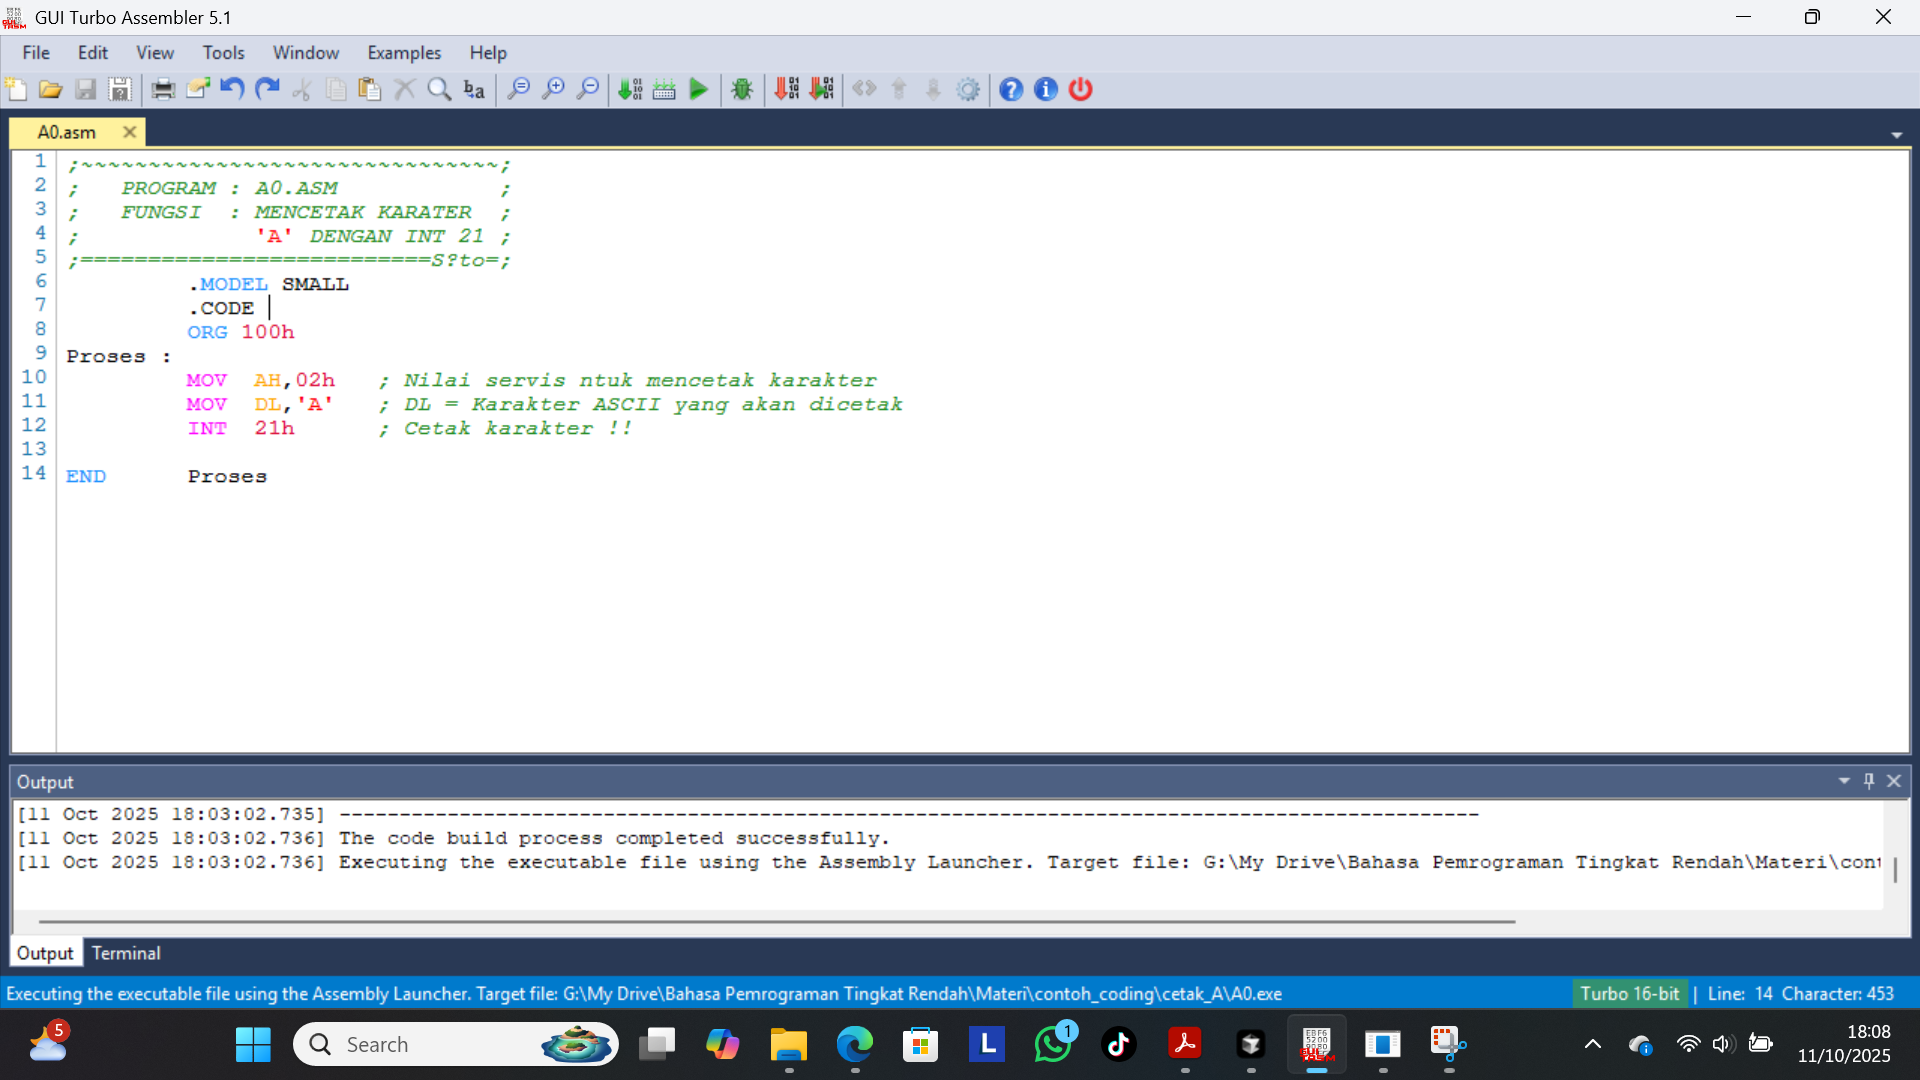
\includegraphics[width=0.85\textwidth]{images/gtasm_build_process.png}
    \caption{Proses build dan run di GUI Turbo Assembler}
    \label{fig:gtasm-build-process}
\end{figure}

            \subsubsection{Membangun Program .COM vs .EXE}
Dalam GUI Turbo Assembler, proses build untuk \texttt{.COM} dan \texttt{.EXE} sama mudahnya:

\textbf{Untuk Program .COM}:
\begin{itemize}
    \item Gunakan model memori TINY dan \texttt{ORG 100h} dalam kode
    \item GTASM akan otomatis mendeteksi dan menggunakan opsi \texttt{/t} pada TLINK
    \item Hasil: file \texttt{.COM} siap dijalankan
\end{itemize}

\textbf{Untuk Program .EXE}:
\begin{itemize}
    \item Gunakan model memori yang sesuai (SMALL, MEDIUM, dll.)
    \item Definisikan prosedur main dengan \texttt{END main}
    \item GTASM akan menghasilkan file \texttt{.EXE} standar
\end{itemize}

\textbf{Catatan}: GTASM secara otomatis menangani parameter TASM dan TLINK yang diperlukan, sehingga tidak perlu mengingat flag command-line yang kompleks.

            \subsubsection{Debugging dengan GUI Turbo Assembler}
GUI Turbo Assembler menyediakan akses mudah ke Turbo Debugger (TD) yang terintegrasi:

\begin{enumerate}
    \item \textbf{Memulai Debugging}:
    \begin{itemize}
        \item Klik tombol \textit{``Debug''} pada toolbar atau menu \textit{``Tools''} $\rightarrow$ \textit{``Debug''}
        \item TD akan terbuka dalam jendela DOSBox dengan program yang sudah dimuat
    \end{itemize}
    
    \item \textbf{Operasi Debugging Dasar}:
    \begin{itemize}
        \item \texttt{F7} atau \texttt{T}: Trace/Step into - eksekusi instruksi per instruksi
        \item \texttt{F8} atau \texttt{P}: Proceed/Step over - eksekusi tanpa masuk ke prosedur
        \item \texttt{F4}: Run to cursor - jalankan sampai posisi kursor
        \item \texttt{Ctrl+F9}: Run - jalankan program sampai selesai atau breakpoint
    \end{itemize}
    
    \item \textbf{Memeriksa Register dan Memori}:
    \begin{itemize}
        \item Jendela Register: Tampilkan nilai register CPU (AX, BX, CX, DX, SI, DI, dsb.)
        \item Jendela Memory: Periksa isi memori pada alamat tertentu
        \item Jendela Stack: Lihat isi stack
        \item Jendela Watches: Monitor variabel atau alamat memori tertentu
    \end{itemize}
    
    \item \textbf{Breakpoint}:
    \begin{itemize}
        \item Tekan \texttt{F2} pada baris yang diinginkan untuk set/clear breakpoint
        \item Program akan berhenti saat mencapai breakpoint
        \item Periksa status register dan memori saat breakpoint tercapai
    \end{itemize}
\end{enumerate}

\begin{figure}[H]
    \centering
    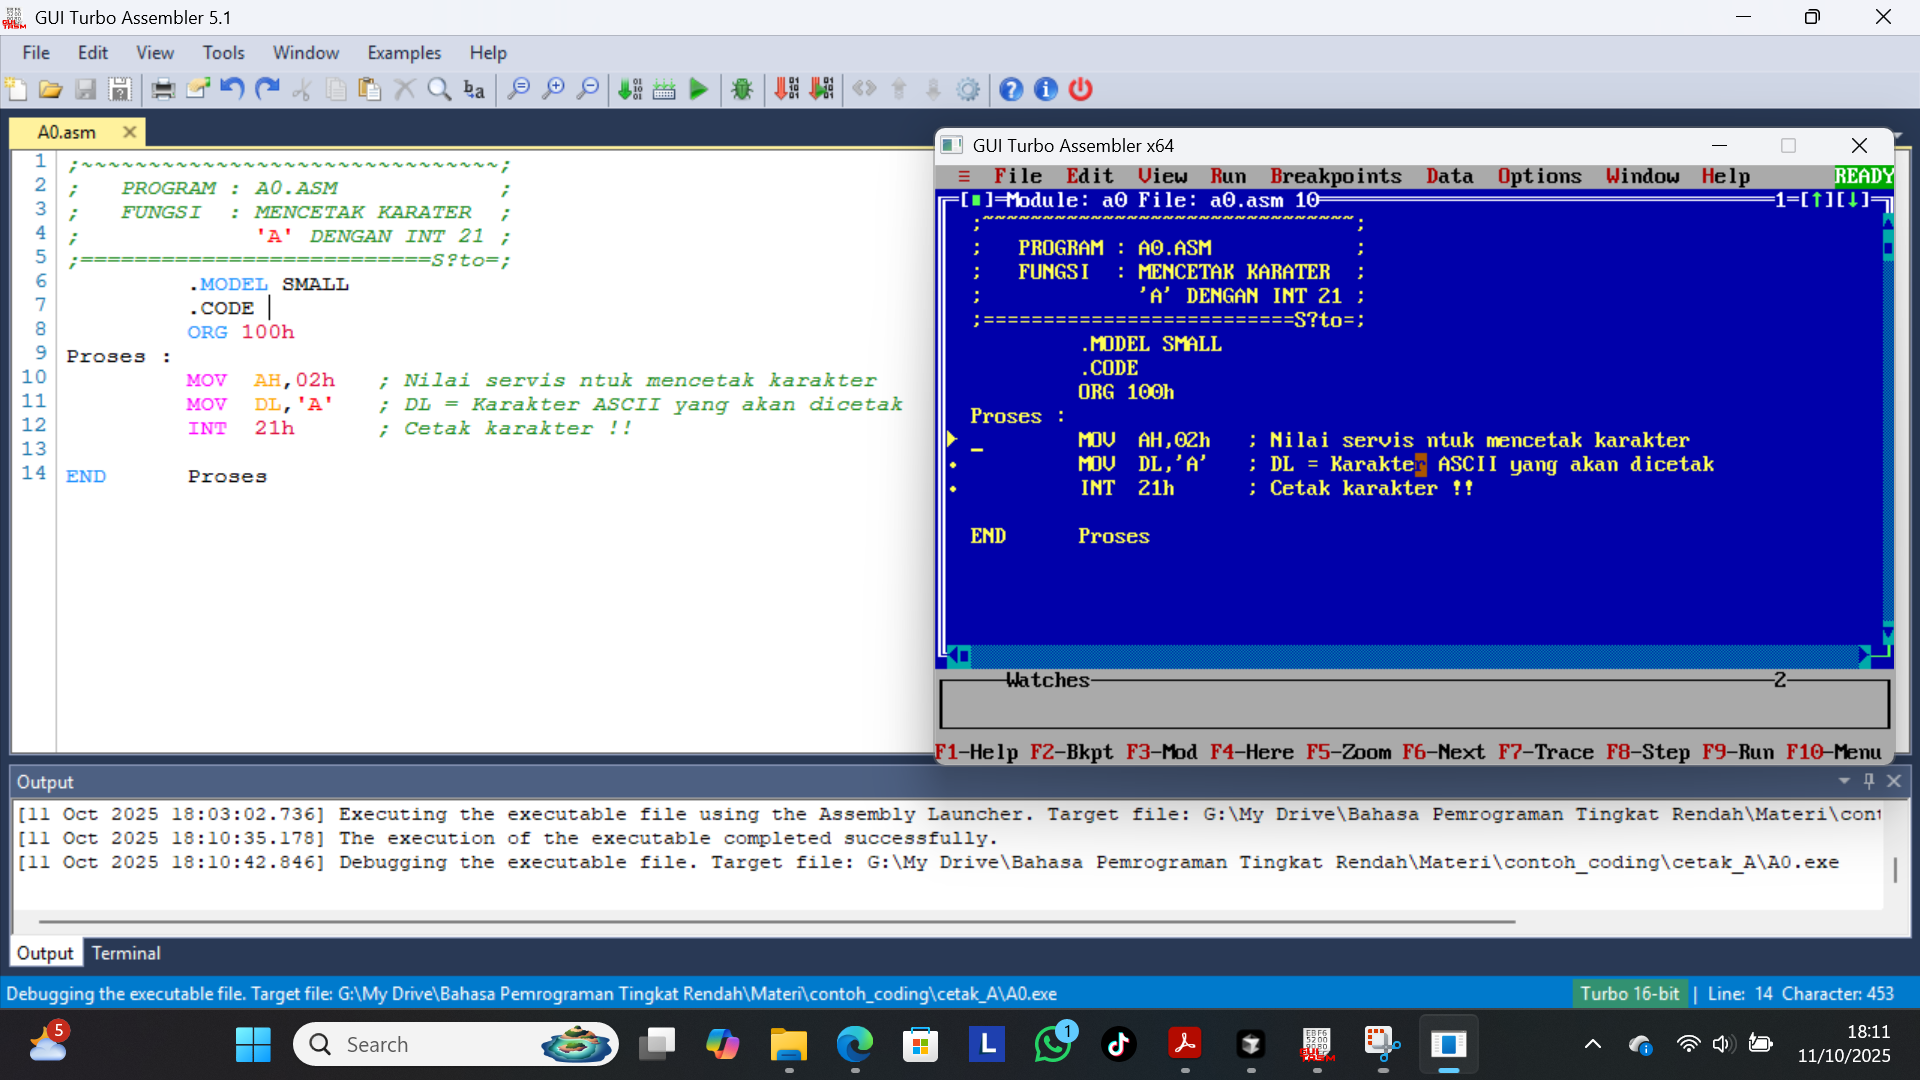
\includegraphics[width=0.85\textwidth]{images/gtasm_debugger.png}
    \caption{Turbo Debugger dalam GUI Turbo Assembler}
    \label{fig:gtasm-debugger}
\end{figure}

            \subsubsection{Kesalahan Umum dan Solusi}
\begin{itemize}
    \item Label tidak terdefinisi: periksa ejaan, urutan definisi, atau kebutuhan \texttt{EXTRN}/\texttt{PUBLIC} (untuk proyek multi-berkas).
    \item \texttt{CS:IP} tidak benar pada program \texttt{.COM}: pastikan \texttt{ORG 100h} didefinisikan dan tidak ada segmen tambahan.
    \item String untuk \texttt{AH=09h}: pastikan terminator karakter \texttt{'}\$\texttt{'} hadir; untuk \texttt{INT 10h} tidak diperlukan.
\end{itemize}





\end{document}
